\documentclass[10pt]{article}
\usepackage[margin=0.85in]{geometry}
\usepackage{amsmath,graphicx,booktabs,hyperref}
\hypersetup{colorlinks=true,urlcolor=blue}
\title{Measured Verification Costs for Speculative Decoding\\\large Expanded experimental results}
\author{Angelina Quan}
\date{November 14, 2026}
\begin{document}
\maketitle
\begin{abstract}
We test a small change to the cost model of an existing adaptive speculative-decoding scheduler: retain measured target-verification costs instead of their monotone envelope. Two expanded studies show modest throughput gains over a globally tuned fixed verification width and native adaptive verification. At batch 64, the gains are 2.56\% and 3.17\%, respectively. Improvement over stronger, prespecified domain-specific fixed widths remains inconclusive. These results support a cost-model ablation in one serving configuration; they do not establish a new scheduler or a benefit from online confidence calibration.
\end{abstract}
\section{Question and intervention}
A scheduler needs estimates of both token acceptance and verification time. Improving confidence calibration can have little effect when it does not change the chosen length. We isolate the cost estimate while keeping the released confidence head and scheduler unchanged.

Let $m(n)$ be the median measured target forward time at profiled token count $n$. The native table applies a cumulative maximum to these measurements. Our variant retains $m(n)$, using the next profiled size for intermediate token counts, up to the CUDA-graph capture limit. The draft-cost table and target costs above that limit remain unchanged. This preserves measured nonmonotonicities that may affect the scheduler's choice. The experiment tests this specific table substitution; it does not claim that nonmonotonic GPU costs or adaptive verification are new discoveries.
\section{Experimental setup}
We use Qwen3-4B with the released DSpark Qwen3-4B block-7 drafter, vLLM 0.33.0, and one H200 GPU. Decoding is greedy with a 128-token output cap. All methods use FP32 tensors, batch-invariant Triton attention, disabled prefix caching, and a 2,048-token context limit. Strict IEEE arithmetic throughout the kernel stack is not established.

The batch-32 study uses 384 prompts; the batch-64 study uses 768 different prompts. Each has equal numbers of conversation, mathematics, and code prompts from Alpaca, GSM8K, and MBPP. The latter study expands MBPP from the sanitized subset to the full official test split, excluding previously used task IDs and normalized text. Prompts were unused at the launch of each expanded study. Subsequent reuse does not create additional independent test data.

Fixed widths are selected on separate exploratory sweeps over widths 1--7. Global width 7 is selected for both studies. The stronger batch-64 comparator uses width 3 for conversation and width 7 for mathematics and code, selected before the expanded run. Each study has four balanced engine orders and two timed passes per session after two full passes for correctness and warmup. Every output in every pass must match the ordinary-decoding reference. Initialization and profiling are outside the timed generation calls; gains describe warmed-up generation throughput, not startup latency.
\section{Expanded results}
\begin{center}
\resizebox{\linewidth}{!}{\begin{tabular}{rrlrr}
\hline
Batch & Prompts & Baseline & Gain (\%) & 95\% CI (\%) \\
\hline
32 & 384 & Tuned global fixed width & +1.25 & [+0.90, +1.59] \\
32 & 384 & Native adaptive & +1.35 & [+1.07, +1.63] \\
64 & 768 & Tuned global fixed width & +2.56 & [+0.85, +4.27] \\
64 & 768 & Native adaptive & +3.17 & [+1.13, +5.45] \\
64 & 768 & Prespecified domain-specific fixed widths & +1.24 & [-1.20, +3.94] \\
\hline
\end{tabular}
}
\end{center}
Intervals are paired, domain-stratified batch-and-round bootstrap intervals (10,000 draws). Repeats stay together; identical prompt groups and rounds are resampled across methods. Gain is $100(T_b/T_m-1)$, where $T_b$ and $T_m$ are aggregate baseline and measured-cost generation times for identical output-token counts. It is not the percentage reduction in latency.

All output checks passed in all 16 sessions in each study. At batch 64, measured-cost throughput is 6,250.80 tokens/s, versus 6,095.03 for global fixed width 7 and 6,058.87 for native adaptive verification. The domain-specific comparator achieves 6,174.37 tokens/s. Its interval crosses zero. The prespecified 5\% mixed-workload target failed. Earlier exploratory chat gains around 10--15\% did not reproduce at that magnitude against stronger baselines.
\begin{center}
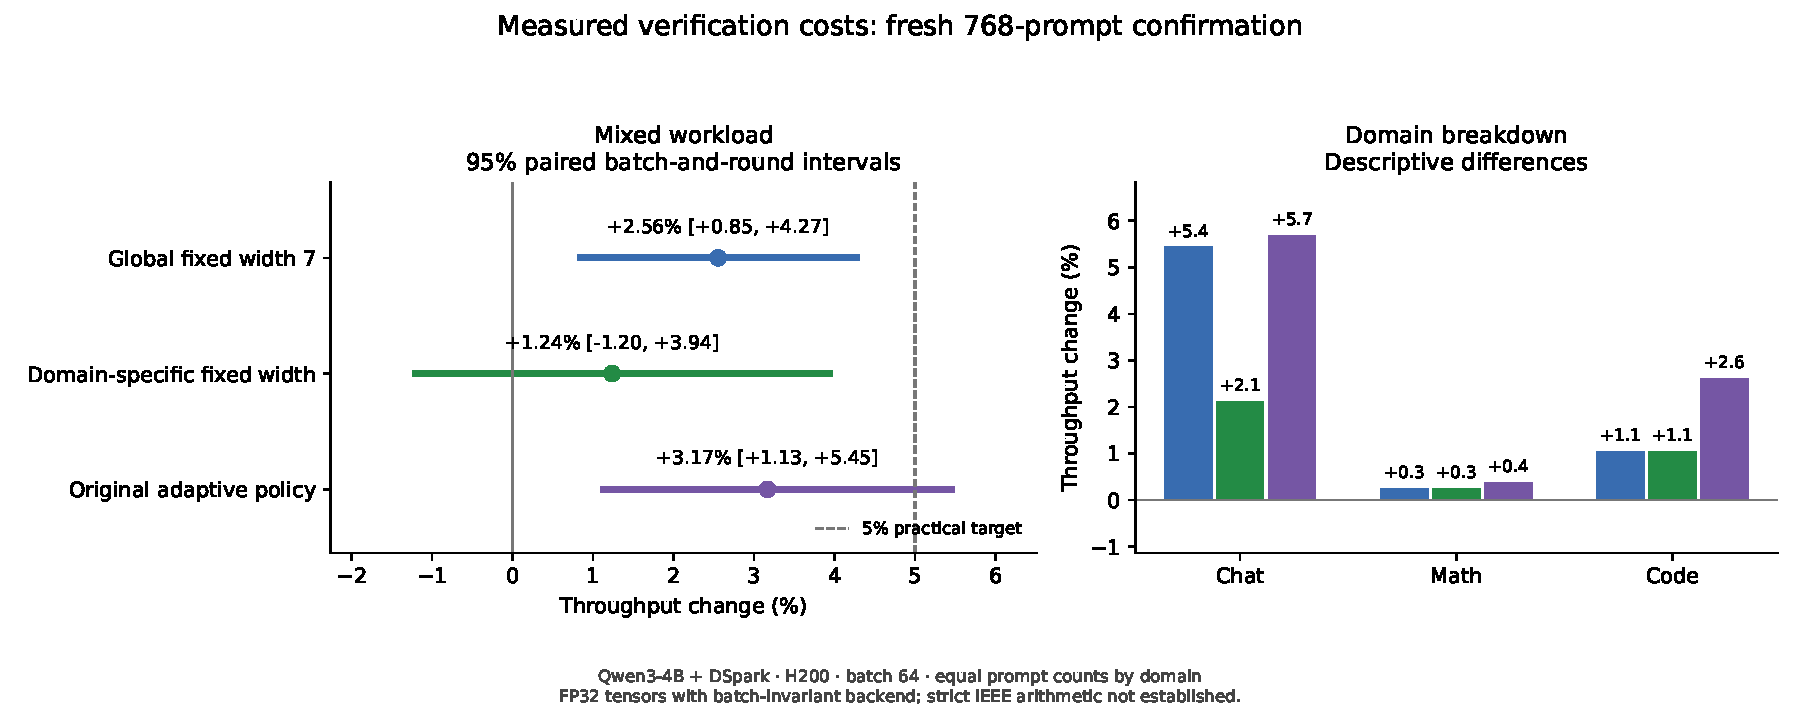
\includegraphics[width=.88\linewidth]{../docs/figures/cost_v38_confirmation.pdf}
\end{center}
\section{Interpretation and limits}
The supported finding is a modest benefit from changing the target-cost table in this configuration. Online calibration pilots did not show a meaningful additional speed gain; these results must not be attributed to calibration. Domain findings are descriptive: batch-64 gains against the prespecified domain baseline are 2.12\% for conversation, 0.25\% for mathematics, and 1.05\% for code.

There are only four prompt batches per domain at batch 64 and four engine rounds. Intervals do not cover uncertainty across devices, model pairs, backends, or workload families, and are not adjusted for the broader exploratory search. A targeted batch-128 sweep is in progress; no result from it is included here. Any expansion on the existing 768-prompt suite will be labeled a reused-suite cross-load replication.
\section{Reproducibility}
The repository contains frozen plans, prompt manifests, output tokens, per-batch timings, source hashes, analyzers, and W\&B links. The table is generated by \texttt{scripts/summarize\_cost\_evidence.py}, which checks output parity and source hashes before extracting audited comparisons. Independent analysis reproduced the batch-64 summary and reconstructed all eight adaptive target-cost tables from raw profiling samples.

\noindent\href{https://github.com/angelinaquan/adaptive-verification-for-speculative-decoding}{Code and raw results}\quad
\href{https://wandb.ai/aquan-world-model/18657-speculative-pilot/runs/vxw4i4v4}{Batch-32 audit}\quad
\href{https://wandb.ai/aquan-world-model/18657-speculative-pilot/runs/az4k5l1i}{Batch-64 audit}
\end{document}
